% remember to set these at the start of each chapter
\chapter{The Next Chapter} 
\label{nextChapt} 

%%%%%%%%%%%%%%%%%%


\section{What About Figures}

Figures are dead easy to call. Just call them from within a Figure environment.

\begin{figure}[h] % put figure roughly here, will float though
	\centering
	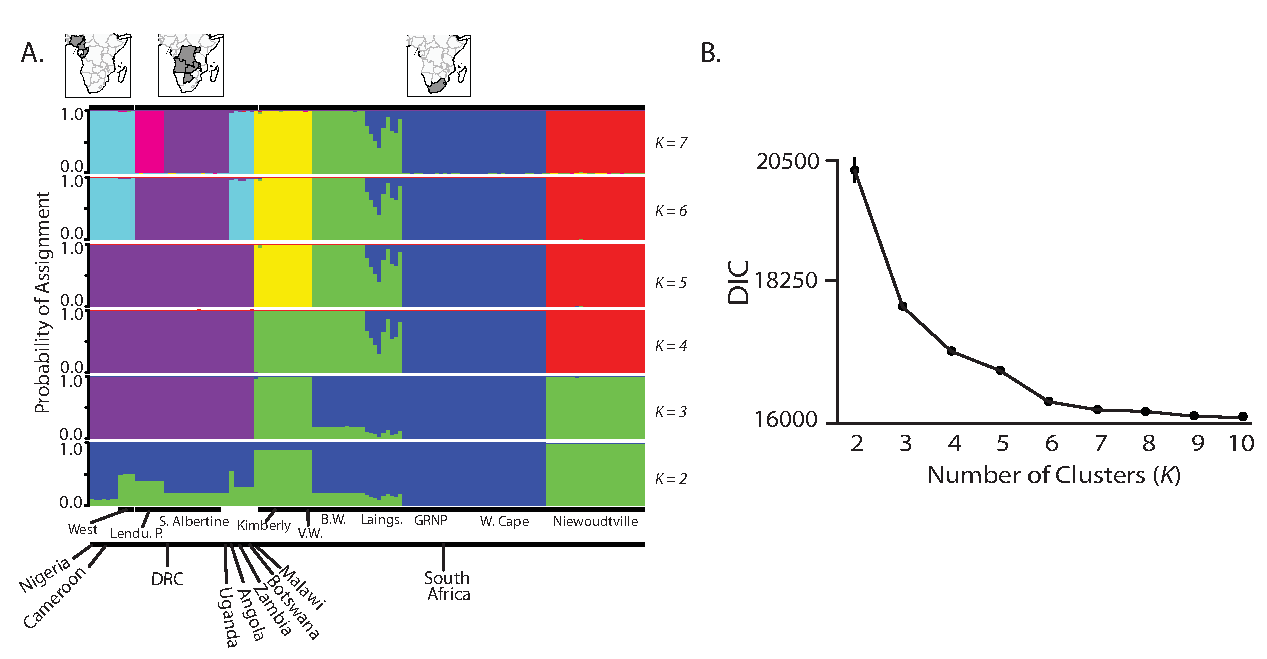
\includegraphics[scale=0.6]{Figs/Fig3_TESS_full_round2.pdf}
    \caption[Admixture]{Genetic structure of populations\ldots}
    \label{tess_analysis}
\end{figure}

And now, I do not need to remember the figure number. All I do is refer to the figure label that I gave it (Fig.\,\ref{tess_analysis}).


As for my next figure, \LaTeX will automatically do the numbering. It will also attach the chapter number to the figure.



\begin{figure}[h!] % put figure roughly here, will float though, h! will strongly suggest where to put it.
	\centering
	\includegraphics[scale=0.6]{Figs/Tree_Fig.pdf}
    \caption[Tree]{A tree of \ac{mtdna}\ldots}
    \label{Tree}
\end{figure}

Then I will call it same as before (Fig.\\,\ref{Tree}). As you can see, it was placed on the next page, as \LaTeX thought that was best, given its size. Figures will float around, but you will never have to worry about numbering. You may notice the \verb+\,+ that just puts in a small space after the Fig. period. \emph{Remember, scalar rendered (Illustrator, Inkscape, R) graphics will not distort! Avoid powerpoint/excel at all costs}. I took a screen shot, which is why these trees look like crap. 

Did you notice that the table of contents/list of figures was all automatically updated too\ldots\.pretty neat. 


\section{Tables -- how to}

\subsection{Typing in Tables}
Small to medium tables I would suggest just typing it in to the \TeX file (see Table \ref{simpleTable} below). There are also packages to create \LaTeX tables (such as xtable in R) and packages to read in csv/tab files, like you read in figures. There are ways to make multi-column and multi-row values in tables; you will have to Google it (it is not hard to do). The \verb+\usepackage{multirow}+ will allow you to do multirow values. The command \verb+\multicolumn{}{}{}+ is already available. 

\begin{table}[h]
\centering
\caption[Simple table]{A simple typed in table. Note the special lines used in the table. Yes, typography rules call for different thickness of lines. The command \\hline will put in just a regular horizontal line}
\label{simpleTable}
\begin{tabular}{c|ccc} 
\toprule
col1 & col2 & col3 & col4 \\
\midrule
1 & 2 & 3 & 4 \\
1 & 2 & \multicolumn{2}{c}{3} \\
\bottomrule
\end{tabular}
\end{table}



% reading in a csv file
\subsection{Reading in CSV table}

You can copy and paste the information into \LaTeX to keep things together, but it has to be dropped into the preamble in the main tex. Or you can call in the data file (Table \ref{csv_readin}).

Using \verb+\usepackage{pgfplotstable}+ is the package to use.

\begin{table}[h]
\centering
\caption[Normal size table]{Reading in a table}
\label{csv_readin}
\pgfplotstabletypesetfile[col sep=comma,every last row/.style={after row=\bottomrule},every head row/.style={before row={\toprule}, after row={\midrule}}]{Tables/Suppl_Table_1.csv}
\end{table}

If tables do not fit, you can shrink them by wrapping in a box or shrinking text (Table \ref{csv_readin_small}).

\begin{table}[h]
\tiny % add text size command 
\centering
\caption[Tiny table]{Reading in a table}
\label{csv_readin_small}
\pgfplotstabletypesetfile[col sep=comma,every last row/.style={after row=\bottomrule},every head row/.style={before row={\toprule}, after row={\midrule}}]{Tables/Suppl_Table_1.csv}
\end{table}

And it is just as easy to rotate tables, and only a little bit difficult to do multi-page rotated tables, any what ever else you want, but packages exist to handle it. 

\section{Clickable Fig/Table refs}

One of the really nice thing about \LaTeX is that the Figure and Table references in text are clickable and will take you to whatever is being referenced (click this number -- Fig. \ref{Another_tree}). There are also commands you can put in to then return, but these are a bit more tricky. 

The same is true for your section headings and the entire table of contents and lists of figures/tables. Additionally, anything that has been given a \verb+\label{}+, when called with a \verb+\ref{}+ will be clickable. 











